%template1.tex
%The following LaTeX source file represents the simplest kind of slide presentation; no overlays, no included graphics. Substitute your favorite style for ``pascal''. To create the PDF file template1.pdf, (1) be sure to use the prosper class, then (2) execute the command latex template1.tex, and (3) the command dvipdf template1.dvi.

%%%%%%%%%%%%%%%%%%%%%%%%%%%%%%% template1.tex %%%%%%%%%%%%%%%%%%%%%%%%%%%%%%%%%%%
\documentclass[a4paper,blends,pdf,colorBG,slideColor]{prosper}
% definitions for slides for CSC544
% Lutz Hamel, (c) 2007

\hypersetup{pdfpagemode=FullScreen}

\usepackage{amssymb}
\usepackage{latexsym}
\usepackage{amsmath}
%\usepackage[usenames]{color}
\usepackage{xypic}


\newcommand{\term}[1]{\ensuremath{\mbox{\bf #1}}}
\newcommand{\nonterm}[1]{\ensuremath{\mbox{#1}}}
\newcommand{\ifstmt}[3]{\ensuremath{{\bf if}\; {#1}\;{\bf then}\;{#2}\;{\bf else}\;{#3}\;\term{end}}}
\newcommand{\whilestmt}[2]{\ensuremath{{\bf while}\; {#1}\;{\bf do}\;{#2}\; \term{end}}}
\newcommand{\funcstmt}[3]{\ensuremath{{\bf fun}\; {#1}\; {\bf is}\; {#2} \; {\bf return}\; {#3}}}
\newcommand{\syntaxset}[1]{\ensuremath{\mbox{\bf #1}}}
\newcommand{\orbar}{\;|\;}
\newcommand{\bs}[1]{\begin{slide}{#1}\ptsize{8}}
\newcommand{\es}{\end{slide}}
\newcommand{\co}{\,\colon\;}
\newcommand{\pair}[2]{\ensuremath{\langle {#1}, {#2} \rangle}}
\newcommand{\encode}[1]{\ensuremath{\langle {#1} \rangle}}
\newcommand{\mytab}{\makebox[.15in]{}}
%\newcommand{\abs}[1]{{\mid{#1}\mid}}
\newcommand{\abs}[1]{{|{#1}|}}
\newcommand{\ol}[1]{\overline{#1}}

\newcommand{\qaccept}{\ensuremath{q_{\mbox{\tiny accept}}}}
\newcommand{\qreject}{\ensuremath{q_{\mbox{\tiny reject}}}}
\newcommand{\accept}{{\em accept}}
\newcommand{\reject}{{\em reject}}

\newcommand{\machine}[1]{
	\begin{quote}
	{#1}
	\end{quote}
	}

\newcommand{\fdef}[1]{
	\begin{center}
	\fbox{
	\begin{minipage}{3.5in}
	{\bf Definition:}
	{#1}
	\end{minipage}
	}
	\end{center}
	}

\newcommand{\ftheorem}[1]{
	\begin{center}
	\fbox{
	\begin{minipage}{3.5in}
	{\bf Theorem:}
	{#1}
	\end{minipage}
	}
	\end{center}
	}

\newcommand{\flemma}[1]{
	\begin{center}
	\fbox{
	\begin{minipage}{3.5in}
	{\bf Lemma:}
	{#1}
	\end{minipage}
	}
	\end{center}
	}


\newcommand{\fframe}[1]{
	\begin{center}
	\fbox{
	\begin{minipage}{3.5in}
	{#1}
	\end{minipage}
	}
	\end{center}
	}

\newcommand{\nframe}[1]{
	\begin{center}
	\begin{minipage}{3.5in}
	{#1}
	\end{minipage}
	\end{center}
	}

\begin{document}

\bs{Algorithmic Information Theory}
Consider the following Strings:
\begin{center}
{\scriptsize\tt
0101010101010101010101010101010101010101010101010101010101010101
}

{\scriptsize\tt
1100100001100001110111101110110011111010010000100101011110010110
}
\end{center}

How much information is in each of the strings?  

Intuitively, very little in the first one
because we can describe/compress the string  as $32*{\tt 01}$.

It seems that we can only describe the second string by its own representation, that is,
the only way to describe it is by  repeating its sequence of zeros and ones.  Therefore,
the second string seems to contain more information.

\fframe{We define the quantity of information contained in an object to be the size of that object's smallest representation or description.}

So,
{\scriptsize
\[
\abs{32*{\tt 01}} < \abs{{\tt 1100100001100001110111101110110011111010010000100101011110010110}}
\]
}
\es

\bs{Minimal Description Lengths}
{\bf Observation:} We can use algorithms to describe the structure of strings.

\fframe{We say that $\encode{M,w}$ is a description of some string $x$ if running the machine 
$M$  with $w$ as input results in string $x$, formally
\[
x = \encode{M,w}
\]
}

{\bf Note:} If we assume that we encode all our descriptions and strings as binary sequences and if $w$ is a binary sequence, then 
\[
\encode{M,w} = \encode{M}w
\]
{\bf Example:} A trivial description.  Consider the machine $I$,
\begin{quote}
$I$ = "On input $w$, where $w$ is a binary string:
\begin{itemize}
\item[1.] \accept."
\end{itemize}
\end{quote}
That is, $x = \encode{I,x} = \encode{I}x$.
\es


\bs{Minimal Description Lengths}
\small
\fdef{Let $x$ be a binary string. The {\bf \em minimal length description} of $x$, written
$d(x)$, is the shortest string $\encode{M,w}$ where TM $M$ on input $w$ halts with $x$ on its tape.
The {\bf\em Kolmogorov complexity} of $x$, $K(x)$, is
\[
K(x) = \abs{d(x)}.
\]
}
{\bf Example:} Let,
\[
x = 0101010101010101010101010101010101010101010101010101010101010101,
\]
then consider the machine $M_1$,
\begin{quote}
$M_1$ = "On input $w$, where $w$ is a binary string:
\begin{itemize}
\item[1.] Write the string $w$ $31$ times on the tape right after the input string.
\item[1.] \accept."
\end{itemize}
\end{quote}
Now we have,
$
x = \encode{M_1}01.
$
If we assume that 
$
|\encode{M_1}| < |x| - 2
$
then $d(x) = \encode{M_1}01$ and therefore,
\[
K(x) = |d(x)| = |\encode{M_1}01|
\]
\es

\bs{Minimal Description Lengths}
The next theorem states that repeating a string does not significantly increase the information content
of the overall string.

\fframe{{\bf Theorem:} \[\forall x \exists q [ K(xx) \le K(x) + q ].\]}

{\bf Proof:} Let $d(x) = \encode{N,w}$, that is $\encode{N,w}$ is a minimal lengths description of
of $x$.  Now, consider the machine $M$,
\begin{quote}
$M$ = "On input $\encode{T,s}$, where $T$ is a TM and $s$ is a string:
\begin{itemize}
\item[1.] Run $T$ on $s$ until it halts and produces a string $z$.
\item[2.] Output string $zz$."
\end{itemize}
\end{quote}
Then $xx = \encode{M}\encode{N,w} = \encode{M}d(x)$.  It follows,
\[
K(xx) \le \abs{xx} = \abs{\encode{M}d(x)} = \abs{d(x)} + \abs{M} = K(x) + q,
\]
with $\abs{M} = q$.
$\Box$
\es

\bs{Incompressible Strings}
\fdef{Let $x$ be a string.  We say that $x$ is {\bf\em compressible} if
\[
K(x) < \abs{x}.
\]
and we say that  $x$ is {\bf\em incompressible} if
\[
K(x) = \abs{x}.
\]}
\es

\bs{Incompressible Strings}
\scriptsize
Before moving on we need to prove the following lemma:

{\bf Lemma:} For all $n \ge 1$,
\[
\sum^{n-1}_{i = 0} 2^i = 2^n -1.
\]

{\bf Proof:} By induction on $n$.  The base case for $n = 1$ is easily shown to hold: $2^0 = 2^1 - 1 = 1$.
For the inductive step we assume that the above holds for any $n$ and we show that that implies that
the above equation also holds for $n+1$,
\begin{eqnarray*}
\sum^{(n+1)-1}_{i = 0} 2^i &=& \sum^{n}_{i = 0} 2^i\\
	&=&\sum^{n-1}_{i = 0} 2^i + 2^n \\
	&=& 2^n -1 + 2^n\\
	&=& 2\times2^n -1\\
	&=& 2^{n+1}-1
\end{eqnarray*}
$\Box$
\es

\bs{Incompressible Strings}
\fframe{
\begin{center}
{\bf Theorem:} Incompressible strings of every length exist.
\end{center}}

{\bf Proof:} We only consider binary strings here because any alphabet can be encoded in binary.  Let $n$ be any length,  it follows that there exist
$2^n$ binary strings of length $n$.  However, there only exist
\[
\sum^{n-1}_{i = 0} 2^i = 2^n -1
\]
descriptions of lengths less than $n$.  Given that each description can at most describe
a single string it follows that there exists at least one string that is incompressible.
$\Box$
\es

\bs{$K(x)$ is not Computable}

\fframe{
\begin{center}
{\bf Theorem:} $K(x)$ is not computable.
\end{center}
}

{\bf Proof:} Proof by contradiction.  Assume that $K(x)$ is computable; also assume the binary alphabet.
We can then construct a machine $M$ 
that given a length $n$ will construct all possible binary strings and apply $K(x)$ to each string.
It will halt and return the first incompressible string $s$ it finds.

Observe that the machine $M$ will always halt with an incompressible string $s$ on its output tape (see the previous
theorem).  Observe also that for $n \gg \abs{\encode{M,n}}$ the description $\encode{M,n}$  could serve as a description
for $s$ with,
\[
\abs{\encode{M,n}} < \abs{s} = n
\]
This is a contradiction, since $s$ is incompressible by construction.

Therefore, our assumption that $K(x)$ is computable must be wrong.
$\Box$
\es

\bs{Alg. Info. Theory}


Even though $K(x)$ is not computable, approximations to this function exist
and are very useful.  Consider
\begin{itemize}
\item data compression
\item machine learning
\end{itemize}
\es

\bs{Data Compression}

Data compression is accomplished with a pair of functions, 
\begin{itemize}
\item $E$ for encoding, 
\item $D$ for decoding. 
\end{itemize}
Then, applying the encoding function to some string $s$ gives,
\[
E(s) \mapsto d'(s).
\]
Where $d'(s)$ is an {\em approximation to the minimal description} and is called the {\em compressed archive}.

If we let,
\[
K(x) \approx \abs{d'(x)},
\]
then we can use the encoding function to compute relative complexity measures between strings.

To obtain the original string from a compressed archive we apply the decoding function,
\[
D(d'(s)) \mapsto s.
\]


 
\es


\bs{Machine Learning}
\small
An interesting application of minimal description lengths is in machine learning.  In some sense
this says that learning can be viewed as data compression.
\footnote{This discussion is based on a tutorial by Peter Gr\"unwald, http://www.cwi.nl/$\sim$pdg/ftp/mdlintro.pdf}



\es

\bs{Machine Learning}

A more quantitative definition of machine learning:
\begin{quote}

Given
\begin{itemize}
\item A data universe $X$.
\item A sample set $S$ where $S \subset X$.
\item Some target function (labeling process) $f\co X \rightarrow \{\text{\it true}, \text{\it false}\}$.
\item A labeled training set $D$, where
$
D = \{ (x ,y) \mid x \in S \text{ and } y = f(x)\}.
$
\end{itemize}
Compute a function $\hat{f}\co X \rightarrow \{ \text{\it true}, \text{\it false}\}$ using $D$ such that,
\begin{equation*}
\label{eq:process-model}
\hat{f}(x) \cong f(x),
\end{equation*}
for all $x \in X$.
\end{quote}

This definition of machine learning is referred to as {\em supervised learning}
due to the fact that the algorithm needs a labeled dataset $D$.

{\bf Observation:} We can view the function $\hat{f}$ as a {\em model} or {\em approximation}
of the original function $f$.  The model is computed only based on the 
observations in the training dataset $D$.
\es
 
\bs{Machine Learning}
One way to compute $\hat{f}$ is to detect regularities in the training set $D$ and describe these
regularities as patterns.

Now, it can be shown that there is a trade-off between learning all the regularities in the training set
and model error.  If we learn the training set too detailed then we obtain an overfitted model
that does not generalize well.

Another way of saying these complex models do note generalize well.

\begin{center}
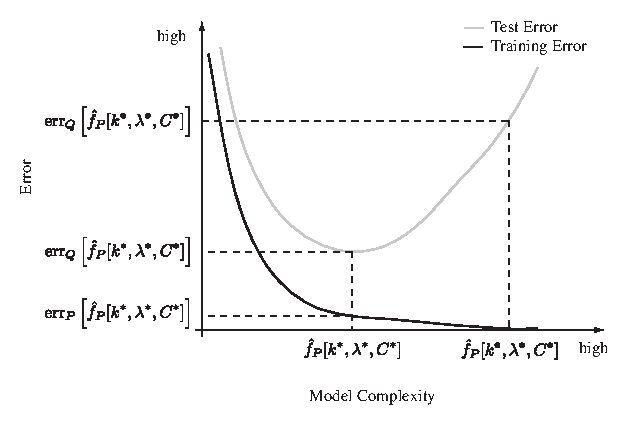
\includegraphics[height=40mm]{images/fig09-02.eps}
\end{center}

\es


\bs{Machine Learning}

Consider the following, we have a simple two dimensional data set, $X$, and we want describe
the relation between the two variables.  A linear model is the simplest and obvious choice, but
it will most likely commit many errors.

\begin{center}
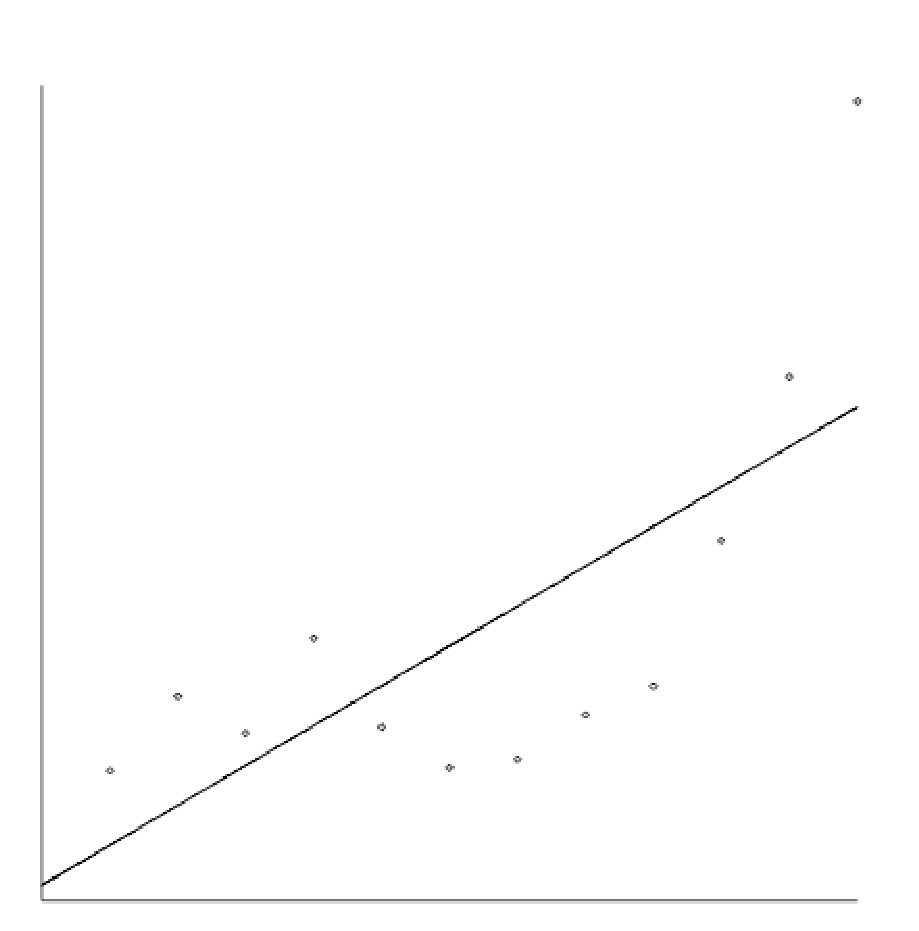
\includegraphics[height=40mm]{images/linear.eps}

(a)
\end{center}

\es

\bs{Machine Learning}
We could try higher order polynomials to see if they fit the data better.

\begin{center}
(b)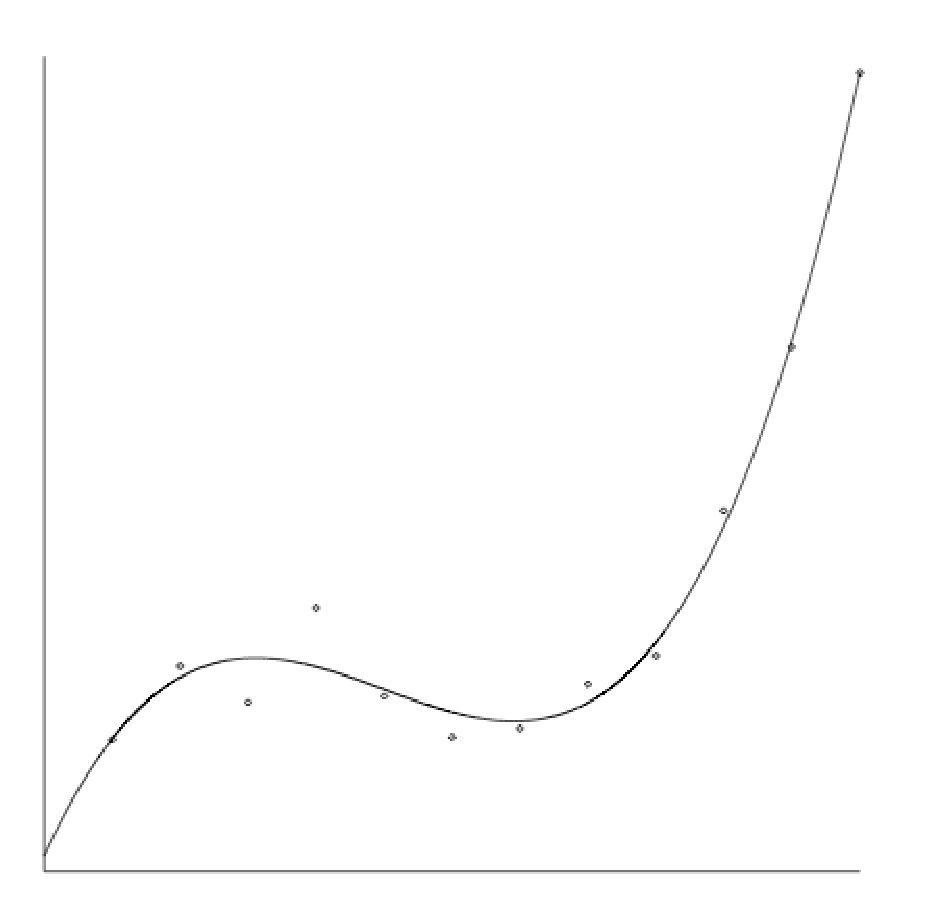
\includegraphics[height=40mm]{images/low-poly.eps}
\hspace{.2in}
(c)\includegraphics[height=40mm]{images/high-poly.eps}
\end{center}

Here (b) commits some errors and (c) commits no errors.

We would consider model (c) more {\em complex} than (b).
\es

\bs{Machine Learning}
\vspace{.2in}
{\bf Observation:} Assuming that $X$ is only a sample from a larger population, there is a tradeoff between 
a model's ability of fitting the {\em training set} $X$ and being able to able to generalize to points
that are not in the training set.  This phenomenon is called {\em overfitting}.  

To avoid overfitting we want to tradeoff model complexity and error rate on the training set $X$.
This process is usually referred to as {\em model selection}.

$\Rightarrow$ One way to address this tradeoff is by using maximal description lengths.
\es


\bs{Machine Learning}
\small
Consider the following.  We can represent the data using models as follows,
\[
\abs{d(X)} = \abs{d(m)} + \abs{d(\varepsilon)}
\]
where $m$ is a model and $\varepsilon$ is an error term that describes on which elements of $X$
the model made a mistake.  

Let $m_0, m_1, m_2$ be the linear, medium powered, and high powered models we saw in 
Figures (a), (b), and (c), respectively, then
we have,
\[
\abs{d(m_0)} < \abs{d(m_1)} < \abs{d(m_2)}.
\]
That is, it is easier to describe linear models than it is to describe high powered polynomial
models.

We also saw that $m_0$ committed the most errors and $m_2$ committed none, so,
\[
\abs{d(\varepsilon_2)} < \abs{d(\varepsilon_1)} < \abs{d(\varepsilon_0)}
\]
So, using $m_0$ to encode the data, we have a very simple model, i.e., a small value for $\abs{d(m_0)}$
but the model commits many errors, so $\abs{d(\varepsilon_0)}$ is going to be large.
On the other hand, if we use $m_2$ to encode the data, then we have a complex model, that is, a
large value for $\abs{d(m_2)}$ but a very small value for the error term $\abs{d(\varepsilon_2)}$.
\es


\bs{Machine Learning}

\vspace{.2in}
This lets us state this as an optimization problem where we prefer a model that gives the minimal description length for $X$,
\[
\min \abs{d(X)} = \min_m \left ( \abs{d(m)} + \abs{d(\varepsilon)} \right).
\]
It has been observed that models selected by minimal description lengths do not overfit and have  good generalization behavior.
Or we can paraphrase this as
\fframe{A good approximation of the data is a reasonable model together with its exceptions.}

\es

\bs{Machine Learning}

{\bf Example:} Given a data set $X$, which of the following models is the most appropriate
model for representing $X$ in the minimal length description:
\[
\begin{array}{c|c|c}
\mbox{model} & \abs{d(\mbox{model})} & \abs{d(\varepsilon)} \\ \hline
m_0 &5 & 25\\
 m_1 & 10 & 10\\
 m_2 & 20 & 5
\end{array}
\]
Here we chose model $m_1$, since $\abs{d(X)} = \abs{d(m_1)} + \abs{d(\varepsilon_1)}$ is 
the smallest representation (minimal length description) of the dataset $X$.  This represents an
appropriate tradeoff between overfitting of the data and model complexity. 
\es
\end{document}
%%%%%%%%%%%%%%%%%%%%%%%%%%% end of template1.tex %%%%%%%%%%%%%%%%%%%%%%%%%%%%%%%%

